\documentclass[twoside]{report}
\usepackage{graphicx}
\usepackage{color}
\usepackage{subfigure}
\usepackage{pdfpages}
\usepackage{listings}
\usepackage[inner=3cm,outer=3cm]{geometry}

\begin{document}
\hyphenation{something}

% Found this:
% http://www.astro.uni-bonn.de/~wucknitz/wiki/lib/exe/fetch.php/lbg:lbw1:preamble.tex
\chapter{Long baseline observations with LOFAR}
Observations using international LOFAR baselines have obtained science quality
images with resolution 0.3$''$ and rms noise $0.15$\,mJy\,beam$^{-1}$ at
154\,MHz, see for example \cite{varenius2014}. In this chapter we will describe
the similarities and differences in the observations and subsequent processing
as compared to LOFAR imaging using shorter (NL) baselines. This chapter is
meant to serve as a reference for you who want to plan observations or
calibrate and image LOFAR data using the longest LOFAR baselines. 
\footnote{The authors of this chapter are Eskil Varenius ({\tt
eskil.varenius@chalmers.se}) and Javier Moldon ({\tt moldon@astron.nl}) with
many useful contributions from the Long baselines working group.}
In section \ref{sect:theory} we give a brief theoretical background and
introduce concepts and vocabulary relevant for long baseline LOFAR observations. 
In the following section \ref{sect:handson} we list practical commands, examples
and code refereces to assist in your calibration and imaging of LOFAR data. 
In section \ref{sect:sched} we summarise the most important points
to remember when scheduling long baseline observations.
Please note that in this chapter, the term \emph{long} baselines refers to international LOFAR
baselines (i.e. length $~1000$\,km) unless stated otherwise. We often use the term NL-LOFAR
to refer to baselines including remote stations within the Netherlands, i.e. baselines of 
lengths $<$121\,km. 

\section{Long baseline interferometry}
\label{sect:theory}
%- Key differences between short- and long-baseline interferometry. Scales for LOFAR VLBI: resolution and field of view.
The prime reason to use long baselines is to obtain very high-resolution images.
Using the longest LOFAR baselines, subarcsecond imaging is possible in the HBA
band and the upper part of the LBA band, see Table \ref{tab:res}.  However, the
wide separation of stations means that each station sees a (very) different
atmosphere, which means that visibility phases are generally less well behaved
than on shorter baselines looking through a more similar patch of the
atmosphere. Further more, the international stations cannot share the same
clock (as the core stations do) and any offsets and drifts of the clocks will
introduce delay errors between the stations. Finally, effects of visibility averaging
are more prominent on long baselines, meaning that interference effects from 
strong sources in the field (e.g. Cas. A etc.) are greatly reduced thereby simplifying
calibration. 
Because of these differences, a somewhat different calibration strategy is
usually employed when imaging long baseline data than what is commonly used for
LOFAR observations with shorter baselines. This need is nothing fundamentally
new for LOFAR, in fact we may borrow many tools and knowledge developed for
decades for use in very long baseline interferometry (VLBI) at centimeter
wavelengths. 

\subsection{What do we want to image?}
NL-LOFAR observations often aim to image a large area on the sky with moderate
resolution for survey purposes as in the MSSS.  In this case we usually want to
make a single large (a degree or more) image. This is tricky for a number of
reasons, as will be touched upon in more detail below, and is, in fact, the
challenges which the major part of this cookbook revolves around.  In such a
large image, the sky is crowded with emission from different things, and
accurate models of the brightest objects (and in particular the strongest
sources like Cas. A) are required to make random noise limited images. 
However, on longer baselines the situation is different for a number of reasons.
To begin with, we often want to image a particular object (e.g. M82) in great detail,
and this object only subtends a very small (arcminute) part of the sky.
Furthermore, at international baselines we are sensitive only to very compact
emission. Many bright sources are partly resolved already at NL baselines, 
and not much flux density is actually present at international baselines, meaning
that the sky is less crowded and the interferring sources are weaker. 
Finally, since we are interested in one (or many) small fields, we may 
average the data, thereby reducing interference from distant sources
as well as reducing the computation required to calibrate and image the data.
All in all, long baselines are in some ways easier to calibrate and image than NL-LOFAR!

\subsection{Field of view: same, same but different}
The area possible to image in a single LOFAR observation (NL or international) is limited
by several factors such as: 
\begin{itemize}
\item The station beam, i.e. the electric field response of a single LOFAR station limiting the signal to noise ratio 
far away from the pointing center. Although the flux densities of an image can be corrected using a good beam model, 
the lack of sensitivity will then manifest as larger rms image noise far from the phase center. Fundamentally speaking,
the decrease in sensitivity cannot be corrected for, so if your source is weak and far from the phase center, you may 
have to re-observe with another pointing to see it.
This effect is independent of baseline length, however: for long baselines 
we use international stations which are bigger than NL-remote stations, meaning a slightly smaller station beam with FWHM 1-2 degrees at 
HBA frequencies, see Table. \ref{tab:res}. 
\item Geometrical/projection effects, such as W-projection artefacts. These can be corrected for in the imaging process using the AW-imager
when making wide field images. This effect is more serious with long baselines, although fundamentally the same. However, since we are 
usually interested in small-field imaging, we may re-project the visibilites to another phase-center before imaging, decoupling the expensive
projection process from the imaging. 
\item Variations in the atmosphere within the image. If the atmosphere is significantly non-uniform over your sky region of interest,
you may need to use multi-directional calibration algorithms, e.g. SAGECAL, to calibrate your data. This can in principle be done, provided
you have enough bright sources to serve as calibrators in your image, but may be computationally expensive. For long baselines,
we are typically interested in only a few directions, reducing the computational demands.
\item Averaging of visibility data, also referred to as time and frequency \emph{smearing}. This effect reduces the amplitude of sources
far from the phase center and may also distort the shape (typically enlarge them). As for the projection losses, averaging losses are
more prominent at longer baselines. Here we need to take care during the observations, and subsequent initial processing, but if we do
we can actually use the averaging effects to great advantage. By averaging, we reduce the impact of interferring sources, and reduce
the data volume, thereby speeding up calibration and imaging. 
\item Disturbance from bright sources in the sky, e.g. Cas. A and others in the \emph{A-team}. Interferring sources can be removed from the data
provided you have a (very) good model of the soure, through \emph{demixing} or similar procedures offered by the observatory. Interference
from bright source may severely affect your dynamic range even if they are far away from the main beam of the station. This effect
is actually much, much less of a problem on long baselines because we may average the data to greatly limit the field of view around 
the objec(s) we are interested in.
\end{itemize}

Generally, all the effects above need to be corrected for to some extent to
make wide field images. But, when we are interested in one (or many)
smaller parts of the sky and we have long baselines, we can focus on making several
small-field images. Here we can use averaging to our advantage. By averaging
the data, interference from distant (e.g. tens of arcminutes, depend on how
much we average) sources is greatly reduced and calibration and imaging is thus simplified.
However, some care is needed with averaging and therefore we elaborate a bit more on this concept below. 

\subsubsection{Time- and frequency smearing limiting field of view}
Since correlators output a discrete set of visibilities (i.e. samples in time
and frequency), averaging is to some extent always done on interferometric
data. We may also average the data further after correlation to reduce the
computational resources needed for calibration and imaging. Any averaging must
however be done with care.  Averaging a range of samples in time and frequency
together corresponds to averaging over a small parallelogram in Fourier space.
This means some information is lost, and one has to take care to not lose
information that could affect the scientific results. For LOFAR, the standard
\emph{raw} data are delivered from the correlator with resolution 1 second in
time, and 64/channels per subband.  Each subband (using the standard 200\,MHz
clock) is 195\,kHz wide, meaning that the limiting averaging bandwidth is
195/64kHz. This will limit the dynamic range at some distance from the observed
phase center, similar to the station beam effects described above.
A detailed description of the 
averaging losses is beyond the scope of this chapter, we merely quote
the often used results by Bridle \& Schwabb, see \cite{NRAO} chapter 18, who derived two expressions to estimate
the average amplitude loss due to averaging in frequency and time, at 
some distance from the phase center. For frequency smearing, we can use 
their expression 18-24 assuming a square bandpass and circular Gaussian tapering, 
where the reduction in amplitude can be estimated as
\begin{equation}
\frac{I}{I_0} = \frac{\sqrt{\pi}}{2\sqrt{\ln{2}}}\frac{\theta \nu_c}{r \Delta \nu}\mathrm{erf}\left(\sqrt{\ln{2}}\frac{r \Delta\nu}{\theta \nu_c}\right)
\label{eqn:freqloss}
\end{equation}
where $\theta$ is the synthesized beam size (FWHM), $\nu_c$ is the central
frequency of the observation, $r$ is the distance from the phase center, and
$\Delta \nu$ is the bandwidth. Note that the units of $\theta$ and $r$ cancel
if they are given in the same unit. Note also that this expression is in fact
independent of central frequency $\nu_c$ since the synthesised beam also scales with
$\nu_c$, only the bandwidth is important.

For time smearing, we may use their formula 18-43, assuming a 12 hour average over a circular UV-coverage 
with Gaussian tapering:
\begin{equation}
\frac{I}{I_0} = 1-1.22\times 10^{-9}\left(\frac{r}{\theta}\right)^2\tau_a^2
\label{eqn:timeloss}
\end{equation}
where $\tau_a$ is the averaging time in seconds.

What loss to define as acceptable of course depends on your science, in
particular the brightness of your target, but as a general guide one may
tolerate 5\% loss in amplitude due to averaging. Using the standard LOFAR raw
data values, we have calculated the corresponding circle (diameter, to compare
with station FWHM) for different observing frequencies, see Table
\ref{tab:res}. We note that, except for the lowest LBA frequencies, we are 
limited by time averaging, where the 5\% loss diameter is smaller than the 
station beam. Note that this limitation is not present for shorter baselines,
and usually not a cause for worry in NL-LOFAR observations. But, with the longest
baselines, the main restriction may (if you need excellent sensitivity) be
the averaging by the raw data.

\begin{table}[h]
\centering
\begin{tabular}{rrrrrr}
Freq. & $\lambda$ & Int. PSF & Int. station& 5\% loss, 1s& 5\% loss, 64ch/SB\\
(MHz) & (m) & FWHM ($''$) & FHWM (deg) & Diam. (deg) & Diam. (deg)\\
\hline
15 & 19.99 & 3.30 & 19.39 & 11.73 & 4.29\\
30 & 9.99 & 1.65 & 9.70 & 5.86 & 4.29\\
45 & 6.66 & 1.10 & 6.46 & 3.91 & 4.29\\
60 & 5.00 & 0.82 & 4.85 & 2.93 & 4.29\\
75 & 4.00 & 0.66 & 3.88 & 2.35 & 4.29\\
120 & 2.50 & 0.41 & 2.59 & 1.47 & 4.29\\
150 & 2.00 & 0.33 & 2.07 & 1.17 & 4.29\\
180 & 1.67 & 0.27 & 1.73 & 0.98 & 4.29\\
200 & 1.50 & 0.25 & 1.55 & 0.88 & 4.29\\
210 & 1.43 & 0.24 & 1.48 & 0.84 & 4.29\\
240 & 1.25 & 0.21 & 1.29 & 0.73 & 4.29\\

\end{tabular}
\caption{Station FWHM Values taken from \cite[App. B]{vanhaarlem2013}. Loss due
to time- and frequency averaging as calculated using eqns.
\ref{eqn:timeloss} and \ref{eqn:freqloss}. Note that the expression
given for frequency smearing is in fact independent of central frequency since
the synthesised beam also scales with frequency, only the
bandwidth is important.
\label{tab:res}}
\end{table}

\subsection{The \emph{shift + average} procedure}
\label{sect:shift+average}
If we are interested in a single source, like the core of M82 which extends about 1 arcminute on the sky, we may average 
much more. For example, in the case of M82 the data were averaged to 1ch/SB and 10s meaning about 0.5\% loss in amplitude
at 30$''$ from the phase center (thereby giving a FoV of 1 arcminute). 
Note however that when averaging this heavily in frequency or time, it is important to first check if there are large residual rates or delays in the data.
%TODO: REF, how large is large? No rate/delay offsets are given. Perhaps convert to offset with simple formula to allow calculation?
If one is interested in multiple objects within the station beam, on needs to phase-shift (and re-project) the UV-data to each object before averaging.
If M82 was not in the center of my field, but say 3$'$ from the phase center, and I averaged as heavily as above without shifting first, I would
decrease the amplitude of M82 with about 14\%.
The need for imaging multiple objects within the same primary beam has shown to be common enough for the Radio Observatory to implement this 
in the official pipelines. Starting during cycle three, you will be able to request shifting and averaging of data to multiple phase centers within a beam 
as a part of your observation. 

\subsection{Calibration of international LOFAR stations}
%- Description of variables relevant for long baseline interferometry: phase, delay, delay rate.
%- Impact of baseline separation, ionosphere, and source structure on the phase behavior.
%- Calibrators needed in a typical long baseline observation (Dutch array calibrator, primary and secondary calibrators).
%- Differences between cm-VLBI and m-VLBI. To understand the dispersive delay produced by the ionosphere.
Data on long baselines are fundamentally no different from data on short
baselines: calibration means to correct any errors in the visibility amplitudes
and phases which were not included in the model applied when the data were
correlated (such as atmospheric effects).  If your target is very bright, you
may be able to calibrate your data using the target itself.  However, to find
amplitude and phase corrections for the international stations, the target must
be sufficiently bright on the angular scales measured by the baselines to the
international stations.  Because of the high resolution, calibration needs to
be done using either a very compact source so that a point source model is good
enough, or we need a very detailed model of the source structure. A science
target is usually both weak and potentially has complex structure (on
subarcsecond scales), which makes it hard to use for calibration of the
international stations. Therefore, a nearby bright (and preferably compact)
sources is usually observed along with the target. 

The amplitude and phase errors are derived using the calibrator, and the
corrections are then applied to the target before imaging. This is called
phase-referencing, and in ordinary VLBI observations it is usually done by
switching back and forth between target and calibrator since an ordinary dish
can only point in a single direction at once. For ordinary VLBI observations
this requires switching often enough so that the corrections derived for the
calibrator is valid also when observing the target source, but since LOFAR
provides multiple beams, we may observe the calibrator and target
simultaneously, simplifying calibration compared to ordinary VLBI. 

However, the calibrator must also be close enough to the target 
for the corrections derived to be valid also in the direction of the target.
Preliminary investigations indicate that the separation between calibrator
and target should not be larger than 5$^\circ$, preferably closer than 1$^\circ$.
From Chapter 29. in \cite{NRAO} the isoplanatic patch size is given as 3-4$^\circ$
at 4\,m wavelength.
If the calibrator is within a 1-2 degrees from the target,
it is possible to use a single beam and then use the \emph{shift+average} procedure,
described in Sect. \ref{sect:shift+average}, to produce two datasets, one for the 
target and one for the calibrator. 

Finding a strong, compact (or a subarcsecond resolution modelled) calibrator within
1$^\circ$ is challenging, mainly because the sky is largely unknown at LOFAR
frequencies. Efforts are under way to build catalogues of suitable sources at
LOFAR frequencies, but often a good first guess can be found by looking at the
VLBI catalogue at higher frequencies: http://astrogeo.org/calib/search.html.
Often one have to settle for a calibrator which is compact and near the target
but which is not bright enough to calibrate the phase and amplitude separately
for each visibility (i.e. each channel/integration time).  The obvious solution
to increase the signal-to-noise (SNR) is to average the data. For shorter
baselines, one may usually average several channels and time bins together,
provided that the errors because of e.g. the atmosphere does not introduce
phase or amplitude changes within the averaging interval. However, for long
baselines the errors are more serious, for example because of the very
different atmospheres above the stations. The ionosphere may introduce
\emph{delay} errors (phase slope vs. frequency) of several hundred nanoseconds,
which means that the visibility phases will change several cycles within a few
MHz of LOFAR data. Blindly averaging such data will severely reduce the
amplitude of the calibrator signal. If the phase also changes with time there
will be a phase slope vs. time as well, which is referred to as a fringe
\emph{rate}.  This means that simple averaging cannot be done to increase the
SNR. This is usually the case also in cm-VLBI, and to be able to use the weaker
calibrators the VLBI community has developed a technique usually referred to as
\emph{fringe fitting}. 

\subsection{Fringe fitting}
The precedure used to find and correct residual rates and delays is called
\emph{fringe fitting}. A fringe fit is nothing more than a self-calibration
including not only phases and amplitudes, but also derivatives of the phase
with respect to frequency and time.  By doing this, more data can be included
in the fitting process thereby increasing the signal-to-noise, which enables
solutions to be found for weak sources and/or in noisy data. Fringe fitting is
described on example LOFAR data in Sect. \ref{sect:fringecal}. For a more
extensive theoretical background, see \cite{NRAO} Chapter 22 and references
theirin, in particular \cite{thompson}.
% TODO: Include phasing up?


\subsection{Distributing bandwidth on calibrators}
In the M82 observations, we spent equal bandwidth on target and calibrator. This is
in principle not necessary, since the calibrator is bright we can use fewer subbands
on the calibrator and thereby get more subbands i.e. lower continuum noise on the target beam.
To use fringe finding, we need to sample accurately the residual delay/rate slope (and possibly curvature at
low frequencies) present in the data. This can be done with sparse sampling in frequency,
where the optimal coverage is achieved by spreading the subbands as a powerlaw density with
denser placement of subbands at lower frequencies. The advantage of this 
approach is that more bandwidth can be placed on the target. The disadvantage is that
the calibration becomes a bit more demanding. One reason for this is that the UVFITS
format used by AIPS (for running fringe fitting) requires data in all channels.
If we do not have contigouse subband coverage in frequency, we need to insert fake
data and flag that (e.g. using NDPPP, see Sect. \ref{sect:fakedata}) before reading
the data into AIPS. This will cause an increase in data volume which will slow down
processing. Also, spreading the subbands sparsely is always a risk in case your calibrator
is weaker than you think. 
If you want to use the sparse sampling of subbands, we reccommend you take a look
at the paper en titled "Optimum estimate of delays and dispersive effects in
low-frequency interferometric observations"
(http://dx.doi.org/10.1051/0004-6361/200913951) from 2010. This paper analyses
on how to distribute subbands specifically in LOFAR observations for optimal
fringe detection.

\section{Calibration example step by step: The M82 data}
\label{sect:handson}
In this section we will take a look at a practical example: the M82 dataset
published by \cite{varenius2014}. 
These data were taken in project LC0\_026 and observed in two parts to maximise
hour angle coverage during night time: 10 hours taken during the night between
the 20th and 21st of March 2013 and 6 hours taken in the evening of April 5th
2013.  Both the March and April observations included the same 44 LOFAR high
band antenna (HBA) stations: 23 core stations (CS), 13 remote stations (RS),
and eight international (INT) stations. Participating INT stations were DE601,
DE602, DE603, DE604, DE605, FR606, SE607, UK608.

\subsection{Plan of the observations}
The observations were designed to image the galaxy M82 with long baselines.
Although M82 is bright ($>$10\,Jy) at NL-resolution, it is weak and complex
with many compact objects at subarcsecond resolution. This means M82
cannot be used as calibrator itself, and another nearby object was needed.
At international baseline resolution, the nearby galaxy M81 is dominated by 
its AGN, M81*, which is compact, and we chose to include M81, 
0.5 degrees from M82, as a nearby phase calibrator. However,
M81* is known to vary in brightness between about 50-150\,mJy
and we did not know if it would be strong enough to use as calibrator,
even with fringe finding to lower the SNR threshold required. Since
these were one of the first long baseline science observations, we
wanted to be safe and included also an extra calibrator which was compact and
brighter. We chose J0958+6533, about 4 degrees from M82, which we found using the
VLBI calibrator search tool available here: http://astrogeo.org/calib/search.html.
The large angular separation is not optimal, and we cannot expect the phase
corrections to be valid across 4 degress. However, a major part of the
corrections will be the same, so if by finding corrections for the amosphere on
J0958+6533, we should be able to calibrate M81* well enough to see a clear
signal, and then we can improve the corrections further by calibrating using
M81* itself before finally transferring the calibration corrections to M82.
This is a two-step phase-referencing process, where we use two calibrators to
find good and better corrections before imaging the target. 

\subsubsection{Dividing the bandwidth}
We aimed to observe at two continuum bands, at 118\,Mhz and at 154\,MHz.
Unfortunately the shift+average approach (sect. \ref{sect:shift+average}) was not
available when these observations were performed, and therefore we 
had to divide the available bandwidth in three separate beams, one on M82, one
on M81* and one on J0958+6533. Today, we would still need a separate beam
on J0958+6533 since it is far outside the station beam, but we could obtain
the M81* and M82 data from the same beam using the shift+average procedure.
Since we divided the total bandwidth of 96\,MHz (with 200MHz clock at HBA) 
at two continuum bands for three objects, 
we ended up with 16\,MHz bandwidth for M82 at 154\,MHz. 

\subsubsection{Flux calibration}
From the VLBI calibrator catalogue we know that also J0958+6533 may vary in
flux density over time. If we had known the flux density
of this object at our observing frequency, we chould have used it at flux
calibrator directly.  However, we now needed to include a final extra
calibrator to fix the absolute flux scale. We chose to include 3C196, which is
very bright and well known (approx 90 Jy, HEALDREF). Since it is so bright,
we only need a few minutes of data and we chose to observe this source 
for two minutes once every hours. These observations also served to 
make it possible to \emph{phase up the core} if it had been necessary for 
fringe finding, see Sect. \ref{sect:phaseup}.

\subsubsection{Observational summary}
So, to sum up: The plan was to observe 3C196 for two minutes every hour, and 
the rest of the time divide the bandwidth in three beams, placed on M82 (the target)
M81 (nearby but weak calibrator) and J0958+6533 (stronger calibrator further away).
No demixing was necessary, so the pipeline requested after observation was just 
standard flagging, and then averaging to 2s, 4ch/SB before storing in the archive.
We wanted to be safe from large residual delays etc.

The first step we want to do to calibrate the M82 data is to find delay and rate corrections
(fringe finding) using the source J0958. However before wants we have a few needs, 
and I will describe these in detail below. First we need to get the data!

\subsection{Get the data into single MS}
\label{sect:fakedata}
The first thing to do is to get the data. The data was put in the LOFAR long
term archive (LTA) as a lot of separate files. First one needs to download
all the relevant files from the archive. This
takes a while, since the data were stored in 2s, 4ch/SB resolution.
In the LTA the data were stored as one file per subband per hour,
so for the upper 16\,MHz data for J0958+6533 I had to download
and keep track of 81 * 16 = 1296 files for this source. 
The split per hour was done since we interrupted the observations once
every hour with a 2 minute scan of 3C196.
After checking the cookbook and talking with science support,
I converged on the following procedure: First combine all subbands together 
within each 1h block giving 16 MS files, then combine those together to a single MS.

I started trying to combine all subbands, but unfortunately, not all files 
were present because of a few random failing nodes
in the observatory pipeline. Since a few missing subbands is not important here,
I used NDPPP to insert fake data (completely flagged) where the missing subbands were.
Example parset for combining all subbands for the same 1h block:
\begin{lstlisting}
msin = [...,'L118547_SB441_uv.dppp.MS','SB442_MISSING',
        'L118547_SB443_uv.dppp.MS',...]
msin.missingdata=True
msin.orderms=False
msin.datacolumn = DATA
msout = J0958_L118547_154MHZ_HOUR1.MS
\end{lstlisting}
The list of input ms has to be ordered correctly in frequency, then the missingdata flag will fill any non-existent file with fake data
(in this case SB442).
At this point we also averaged the data to 10s, 1ch/SB to speed up the calibration process. 
This was done by adding the following lines to the NDPPP parset:
\begin{lstlisting}
averager.freqstep = 4
averager.minperc=0.0
averager.minpoints=0
averager.timestep=5
averager.type=averager
steps = [averager]
\end{lstlisting}
(Note that the data were previously averaged to 4ch/SB and 2s by the pipeline).
%TODO: Reference delays and rates check 

After running the parset we had 16 MS files for source J0958 at 154MHz, one for each of the 16 hours. These were now combined 
using the task \emph{concat} in CASA:
\begin{lstlisting}
concat(vis=['HOUR1.MS', 'HOUR2.MS', ...], concatvis = 'OUT.MS')
\end{lstlisting}

\subsubsection{For convenience: changing source names}
In subsequent tasks you will often have to specify a source name. By default,
the LOFAR MS will have source names called \verb!BEAM_0! or similar. It is
often hard to remember which source had what beam-index, and therefore it may
be useful to change the source names to something more useful. This can be done
interactively using the task \emph{browsetable} in CASA.  After opening the
task, open the MS, press 'Table keywords' on the left, double click on the row
'FIELD', and then double click on the source 'NAME' column. If you get a
warning that the browser is not in editor mode, you may enter edit mode by
pressing CTRL+E, or use the 'Edit menu' and press 'Edit table'. When you have
changed the source name, close the MS to save the changes.

\subsection{Converting from linearly polarised MS to circularly polarised UVFITS}
Global fringe fitting solving for delays and rates is, when writing this,
only available within the Astronomical Image Processing System (AIPS,
see http://www.aips.nrao.edu). To read the data into AIPS, we first need
to convert from the standard LOFAR format of Measurement sets in alinear (X,Y)
polarisation basis to UVFITS-files in a circular (R,L) polarisation basis. 
This is done in two steps, first the conversion to circular and then the conversion
to UVFITS.

\subsubsection{Conversion to circular polarisation basis}
%- To understand why circular polarization is useful and how to convert the data.
Standard VLBI techniques like fringe fitting work in a circular (R,L)
polarisation basis. In this basis, the ionospheric disturbances are transformed
from coupled amplitude/phase effects (as in the linear X,Y basis) to phase only
effects. Also, since differential Faraday rotation does not mix R and L
polarisations we may calibrate RR and LL independently. Conversion to circular
polarisation may be done using different tools.  The M82 data
\cite{varenius2014} were converted from linear to circular using the tool
\emph{mscorpol} v1.6, developed by T. D. Carozzi.  This tool includes
corrections for dipole-projection effects as a function of the correlated sky
position relative to all included LOFAR stations.  After the conversion, the
data are circularly polarised, with full (but approximated) parallactic angle
correction. 
Normally the script is executed on an MS file to produce dipole corrected data in a
circular basis. The shell command:
\begin{lstlisting}
mscorpol -f INPUTFILE.MS
\end{lstlisting}
produces corrected data in the DATA column. For more info see the mscorpol manual.

\subsubsection{The UV-FITS format}
%- Brief introduction + references to FITS files, convert them, and manipulate them in AIPS.
Since AIPS understands the UVFITS-format, but not Measurement Sets (MS)
we need to convert the data from MS to UVFITS. There are several ways to do this:
\begin{itemize}
\item You may use the function \emph{exportuvfits} in CASA.
\item You may use the tool \emph{ms2uvfits} available at the LOFAR cluster, as {\tt ms2uvfits in=[input-MS] out=[output-FITS-file] writesyscal=False}
\end{itemize}
Note that in a UVFITS file there MUST be data for all baselines included, although
data can be flagged if baselines are bad. If one tries to reduce data size by exluding particular subarrays
with NDPPP one may run into very strange errors in AIPS, since the basic assumptions of UVFITS are not valid.
Hence, it is important to ensure that data are contigous in frequency (e.g. by inserting fake data as explained above)
and that there are data present for all baselines in the dataset. 

\subsection{Loading the data into AIPS}
The AIPS task FITLD can be used to load the data in to AIPS. For LOFAR data,
the parameters digicor=-1 and douvcomp=-1 should be used.

\subsection{Introduction to AIPS tables}
In AIPS one calibrates data by sucessively finding and improving corrections for the 
amplitude and phase of visibilites. These corrections are stored in tables.
Each correction derived is store in an 'SN' table, and the cumulative corrections
are stored in a 'CL' table. The SN table will have a resolution which you specify for each
task, i.e. if you find corrections averaging data in two minute chunks,
the SN table will have one value every two minutes. The CL table may have a different granularity,
so that when applying a specific SN table, you may (automatically) interpolate to 
CL-table entries between the SN entries. When you are done with calibration, the CL-table
including all your corrections can be multiplied with your data using the task SPLIT to produce
a UVFITS file with the corrected data.

In this example we will produce SN tables with the tasks FRING (to find delay/rate corrections)
and CALIB (to find amplitude/phase corrections). These SN tables are applied to the data by
successive application of the specific SN table to the latest CL-table, thereby creating one single
CL table containg all corrections.

\subsection{Fringe fitting}
\label{sect:fringecal}
In AIPS the most commonly used task for this is called \verb!FRING!. This task
considers the first derivatives of phase vs. frequency and time, i.e. it
assumes linear delays and rates within the selected bandwidth and solution
interval.  
%TODO: CURVATURE 
As an example, let's inspect two minutes of data on a particular baseline
(CS001HBA - DE601HBA) for the source J0958+6533, the source used to find and
correct residual delays and rates by \cite{varenius2014}.  The raw-data is
plotted using the AIPS task \verb!POSSM!  in Fig. \ref{fig:J0958Hprefring}.
From this figure we can see by eye that the phase $\phi$ changes approximately
$\Delta \phi=1.5$ cycles (i.e.  $1.5\cdot2\pi$ radians) over the full bandwidth
of $\Delta \nu=$15.9\,MHz.  Assuming a linear phase gradient we can estimate
the delay as $\tau = \Delta \phi / \Delta \nu=94$\,ns at this particular time.
Indeed, FRING finds a very similar value as can be seen around 22 UT in
\ref{fig:J0958Hdelays}.  These corrections were found using the default
parameters of FRING, with the following manual changes: The search was
restricted to baselines longer than 60k$\lambda$ (\verb!uvrange = 60,0!), a
delay search window of 600\,ns (\verb!dparm[2]=600!), a rate search window of
30\,mHz (\verb!dparm[3]=30!), and a solution interval of 2 minutes
(\verb!solint=2!).  Solutions were found separately for each IF and
polarisation. A ParselTongue code snippet (see Sect. \ref{sect:parseltongue})
doing this is:
\begin{lstlisting}
fring=task('fring')
fring.indata = data
fring.docalib = 1 # Use any previous calibration,
                  # not relevant since this is first
                  # cal step, but in case one derives
                  # other corrections before, this need
                  # to be included
fring.gainuse = 0 # Use highest CL version
fring.calsour = [None, 'J0958']
fring.refant = 1 # Reference antenna.
fring.snver = 1 # The output SN table version
fring.solint = 2.0
fring.dparm[2] = 600 # ns delay window
fring.dparm[3] = 30 # mHz, for speed
fring.uvrange = [None, 60, 0] # use only long baselines
fring.go()
\end{lstlisting}


\begin{figure*}[htbp]
\centering
\subfigure[Before fringe fitting]{
    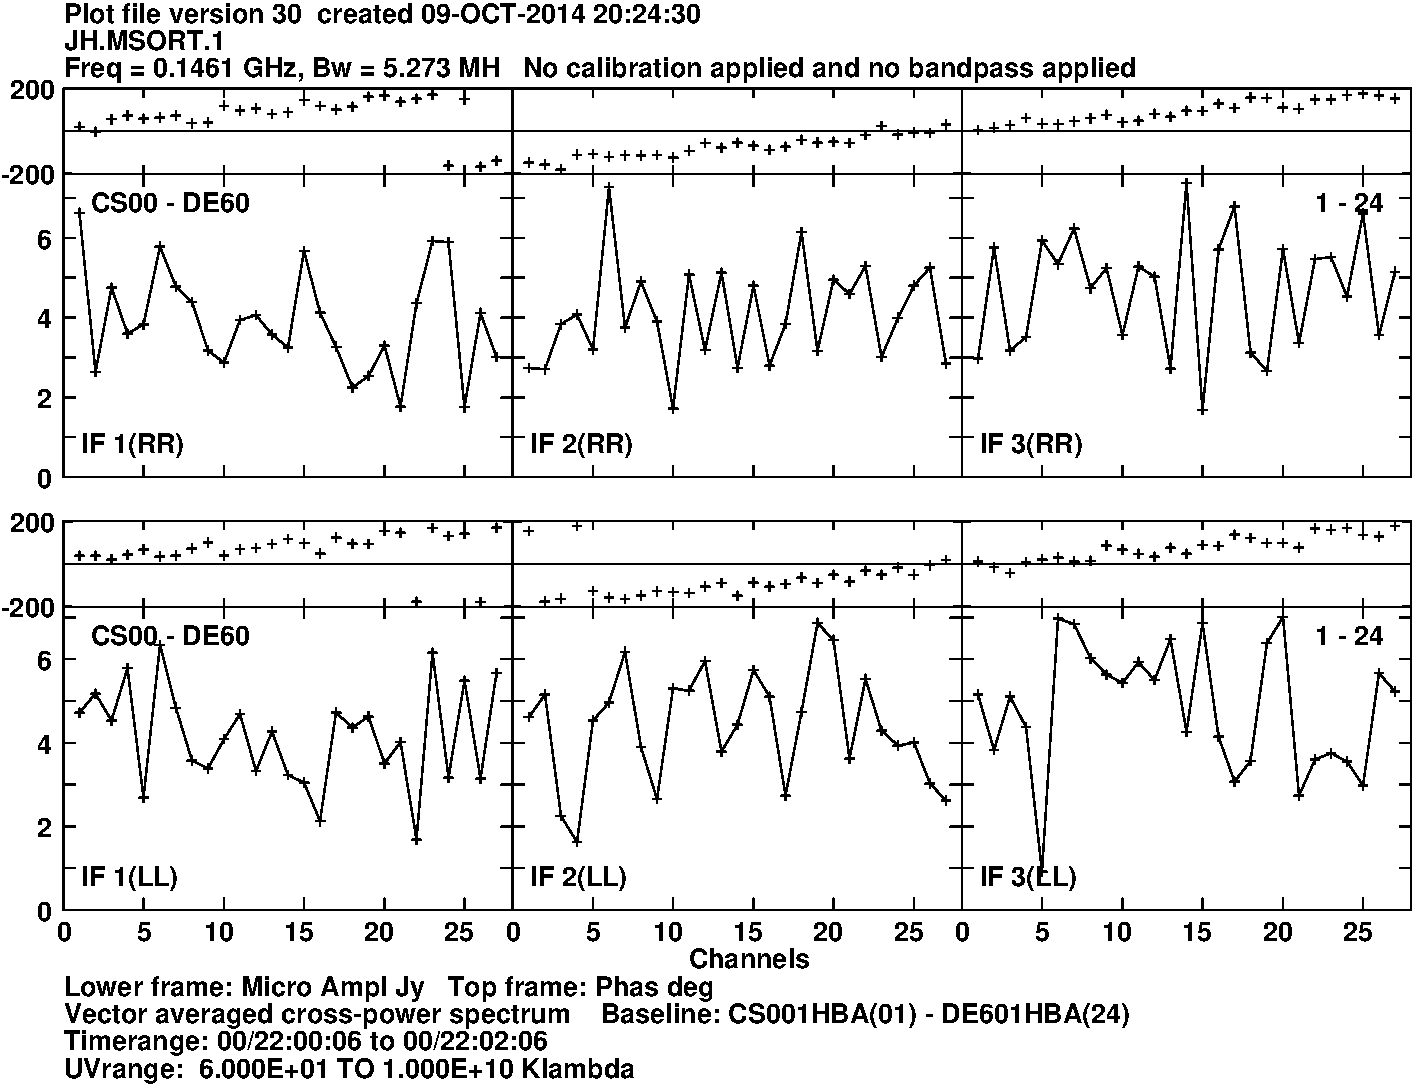
\includegraphics[width=0.7\textwidth]{figs/J0958Hprefring-crop.pdf}
    \label{fig:J0958Hprefring}
}
\subfigure[After fringe fitting]{
    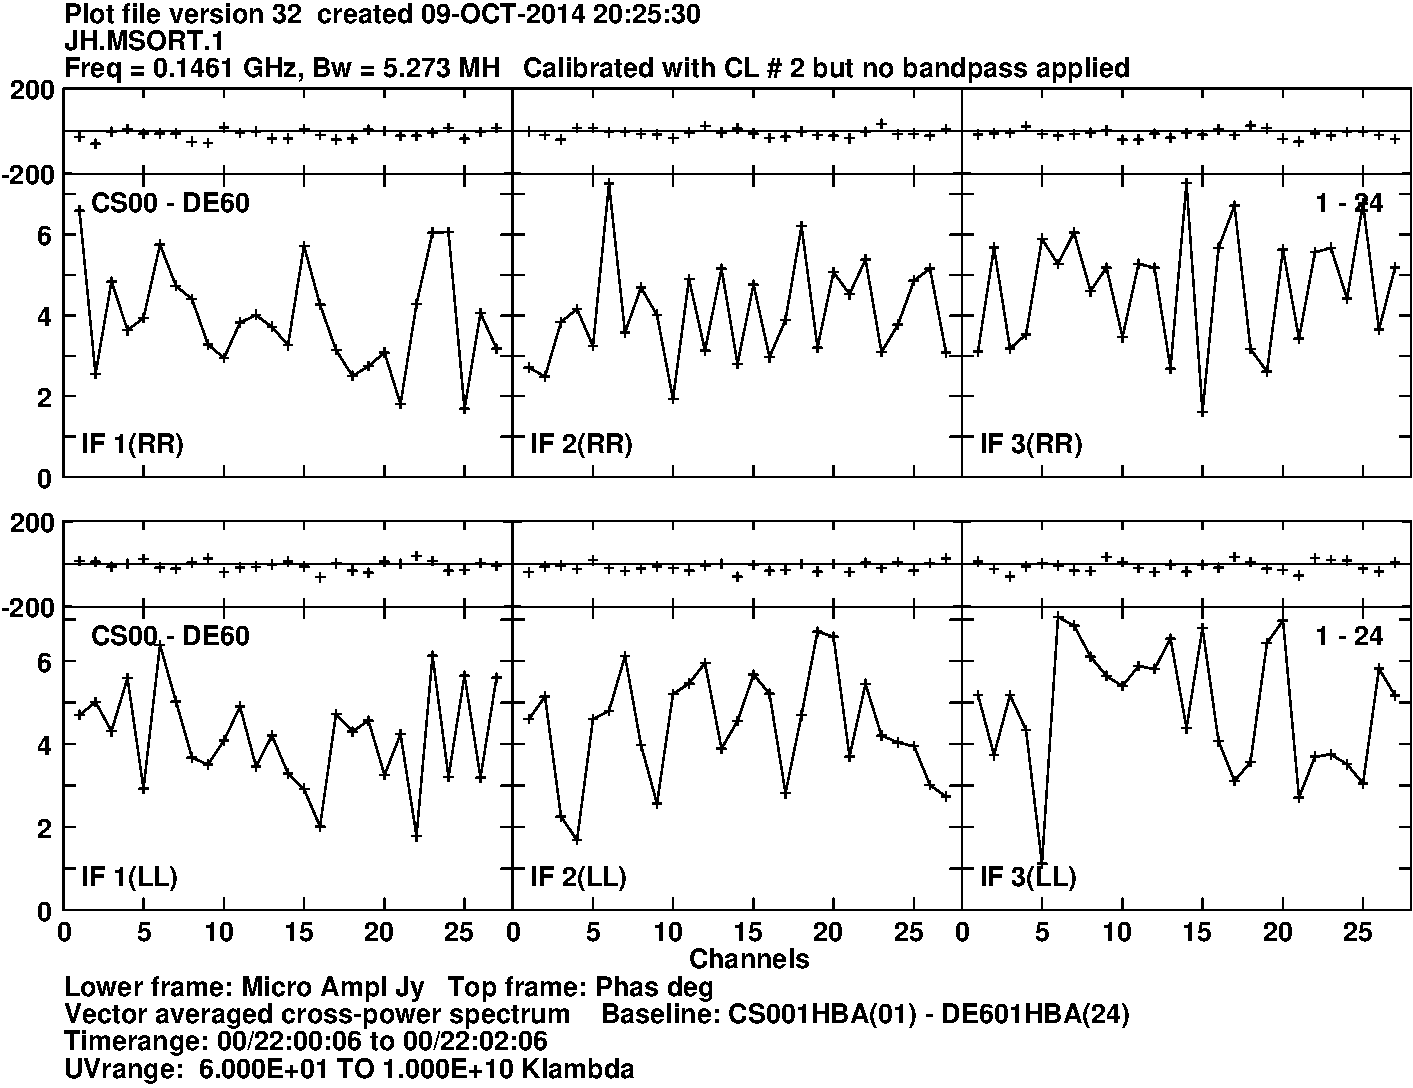
\includegraphics[width=0.7\textwidth]{figs/J0958Hpostfring-crop.pdf}
    \label{fig:J0958Hpostfring}
}
\caption{
Two figures showing the effect of fringe fitting on two minutes of data on the baseline CS001HBA - DE601HBA. Both 
polarisations are shown, and the data are divided in three spectral windows (IFs in AIPS) of 5.3\,MHz each. 
After applying the corrections from FRING,
the phase is flat with respect to frequency, see \subref{fig:J0958Hpostfring}, as it should be for a point source.
\label{fig:fringex}
}
\end{figure*}

\begin{figure*}[htbp]
\centering
\subfigure[Delay corrections for DE601HBA IF2]{
    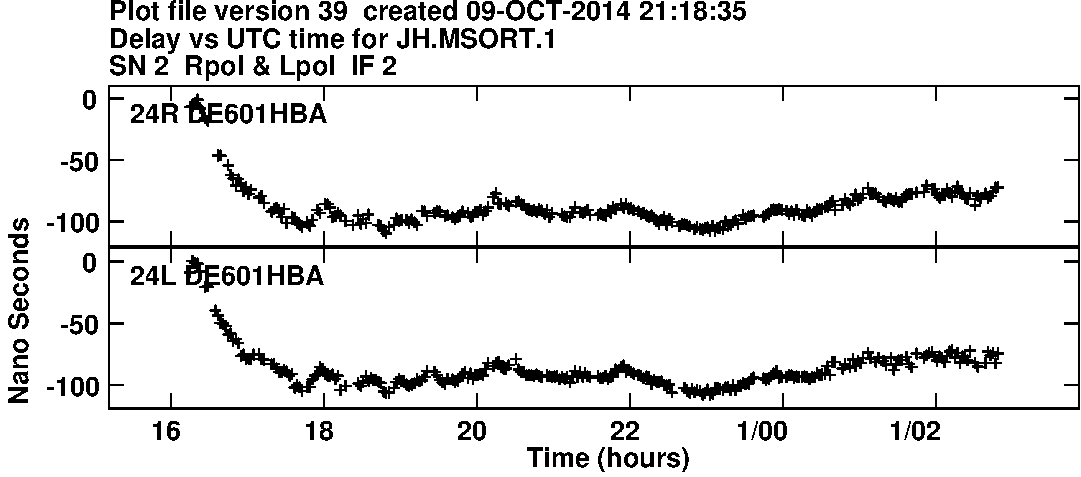
\includegraphics[width=0.75\textwidth]{figs/J0958Hdelays-crop.pdf}
    \label{fig:J0958Hdelays}
}
\subfigure[Rate corrections for DE601HBA IF2]{
    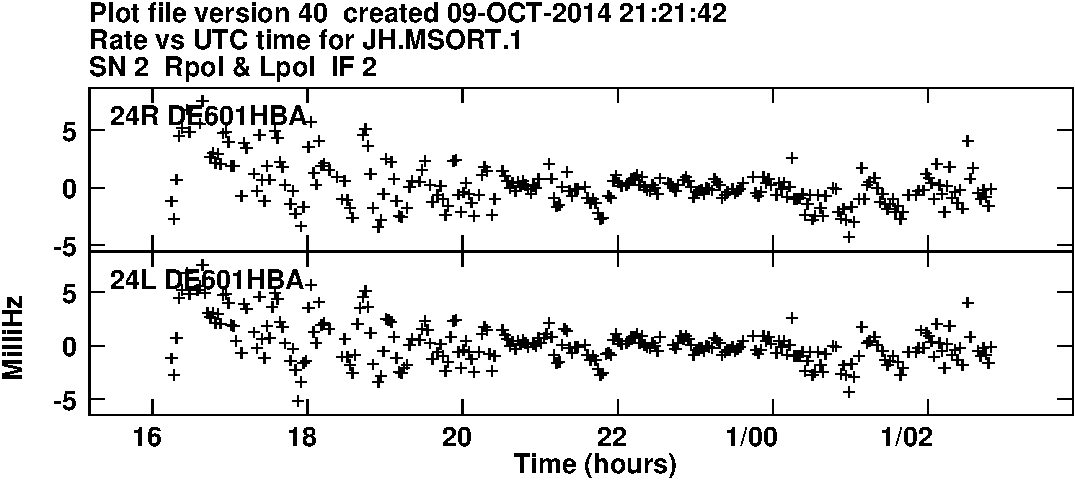
\includegraphics[width=0.75\textwidth]{figs/J0958Hrates-crop.pdf}
    \label{fig:J0958Hrates}
}
\subfigure[Phase corrections for DE601HBA IF2]{
    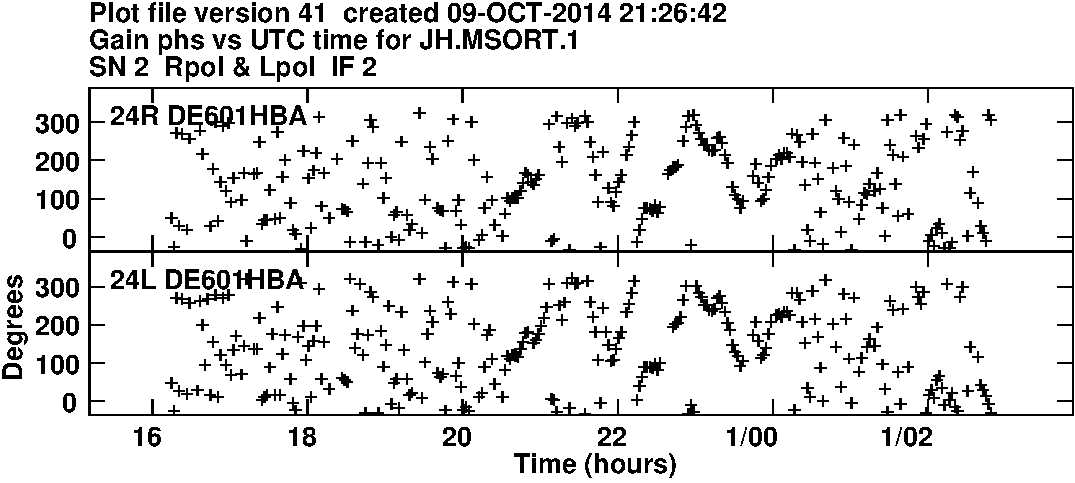
\includegraphics[width=0.75\textwidth]{figs/J0958Hfringpsol-crop.pdf}
    \label{fig:J0958Hfringphases}
}
\caption{
Delay (\subref{fig:J0958Hdelays}), rate (\subref{fig:J0958Hrates}) and phase
\subref{fig:J0958Hfringphases} corrections derived for the source J0958 at 154\,MHz
by FRING for antenna DE601HBA.  These plots show the corrections derived for
the whole 10 hour observation (the first segment of project LC0\_026). It is
clear from the rates and phases that phases changes rapidly during the first
and last hours of the experiment. The delay solutions are more stable, although
there is a large change in at the start. In general, the ionosphere is more
stable during midnight than at sunset or sunrise. 
}
\label{fig:fringsols}
\end{figure*}
Inspect the solutions carefully with SNPLT after use of FRING. The
solutions should be smoothly varying with time, and are typically a
few tens of nanoseconds for most antennas. Large delays (microseconds
or above) should be reported to the Observatory, particularly if they
appear in more than one dataset or if there are sudden changes in
the delay.

\subsection{Smoothing/filtering the solutions}
Sometimes it is desirable to smooth the solutions if they are very noisy, or to
use a median window filter to remove obvious outliers. This can be done with
the task SNSMO. Note however that smoothing the solutions can be very
dangerous, care needs to be taken when doing this to ensure you do not change
the solutions in a way to lock in subtle errors which may affect your
calibration later. 
To remove obivious outliers in the FRING solutions, the following
input to SNSMO was used (given in ParselTongue format, see Sect. \ref{sect:parseltongue})
to smooth the FRING solutions (SN1) for the J0958 calibration:
\begin{lstlisting}
data = UV(NAME, CLASS, DISK, SEQ)
snsmo = task('snsmo')
snsmo.default()
snsmo.indata = data
snsmo.samptype = 'MWF'
# Support times for filter, in hours
snsmo.cparm[2] =  0 # phase
snsmo.cparm[3] =  0.3 # rates
snsmo.cparm[4] =  1.0 # singleband delay
snsmo.cparm[5] =  1.0 # multiband delay
# Clip thresholds
snsmo.cparm[7] =  400 # maxphas, degrees, i.e. no clip based on phase
snsmo.cparm[8] =  10# max rates, mHz
snsmo.cparm[9] =  100 # max single delay, ns
snsmo.cparm[10] =  100 # max multi delay, ns
snsmo.inver = 1 # The SN table to be smoothed
snsmo.outver = 2 # The SN table where to put new solutions.
snsmo.smotype = 'VLBI'
snsmo.refant = 1
snsmo.doblank = -1
snsmo.go()
\end{lstlisting}
This produced SN version 2, which is in fact what is shown in Fig,
\ref{fig:J0958fringsols}. In this case only a few points were removed and the
original version 1 was very similar to after filtering. 

\subsection{Applying the solutions with CLCAL}
Now we have derived (and filtered outliers) delay/rate/phase corrections for J0958, and
saved these in SN table version 2. These solutions now need to be applied to the data,
usint the task CLCAL. An eample ParselTongue code snippet to do this:
\begin{lstlisting}
clcal = task('clcal')
clcal.default()
clcal.indata = data
clcal.snver = 2 # The SN table to apply
clcal.invers = 2 # Again, the SN table to apply. Two lines, since 
                 # CLCAL can apply a range of tables (not used here).
clcal.calsour = [None, 'J0958'] # None needed in ParselTongue syntax, 
                                # since AIPS counts from 1, and python from 0.
clcal.gainver = 1 # Old CL version, containing all corrections before FRING
clcal.gainuse = 2 # New CL table version including also FRING corrections
clcal.refant = 1
clcal.go()
\end{lstlisting}
After applying the corrections from FRING, the phase is flat with respect to
frequency, see \ref{fig:J0958Hpostfring}, as it should be for a point
source.

\subsection{Amplitude calibration: bootstrapping to short baselines}
%- Ways to obtain the amplitude calibration for international stations
As described earlier the calibrator used for deriving delay, rate and phase
corrections need to be close to the target and sufficiently compact to show
enough signal on the longest baselines. This calibrator can in principle also
be used for amplitude calibration of the long baselines, but again a good model
is required. For fringe finding, the only requirement for good solutions is
that the calibrator is bright enough and compact enough.  But, for amplitude
calibration, we must know the flux density of the calibrator.  Usually the VLBI
calibrators stay compact, but the flux density can vary more than a factor of
two between observations due to intrinsic variability. Therefore they cannot be
trusted to set the amplitude scale of the observation. 

For the case of M82, the calibrator J0958 is bright and compact enough for amplitude
calibration of the international baselines, but we did not know the correct flux density. 
Therefore, we included observations also of a known flux calibrator, 3C196. Now, the calibrator J0958
was used to track possible amplitude variations during the observation for all stations, and
3C196 was used to check the absolute amplitude scale, i.e. to find the flux density of J0958. 

The amplitude corrections should be smooth, and will in most cases show a larger gain at the start and end of an experiment.
This is because an observation is usually centered in time so that the target will reach its peak elevation at the middle of the
observation time. This means that it will be at lower elevation in the begining and end of the observation, which means that
the projected station area will be less at the start and end times. This in turn means that the sensitivity is lower at the start
and end times, which means that the gain corrections need to be larger (and will be noisier) at these times. As an example,
let us look at the gain corrections derived by CALIB in AIPS for DE601HBA on J0958, see Fig. \ref{fig:ampcal}.
When running CALIB, we have decreased the number of free parameters compared to FRING, since we are now only solving for amplitude and phase. 
It is therefore possible to find minor phase corrections at this point which was not perfectly determined by FRING.

\begin{figure*}[htbp]
\centering
\subfigure[Amplitude corrections for DE601HBA IF2]{
    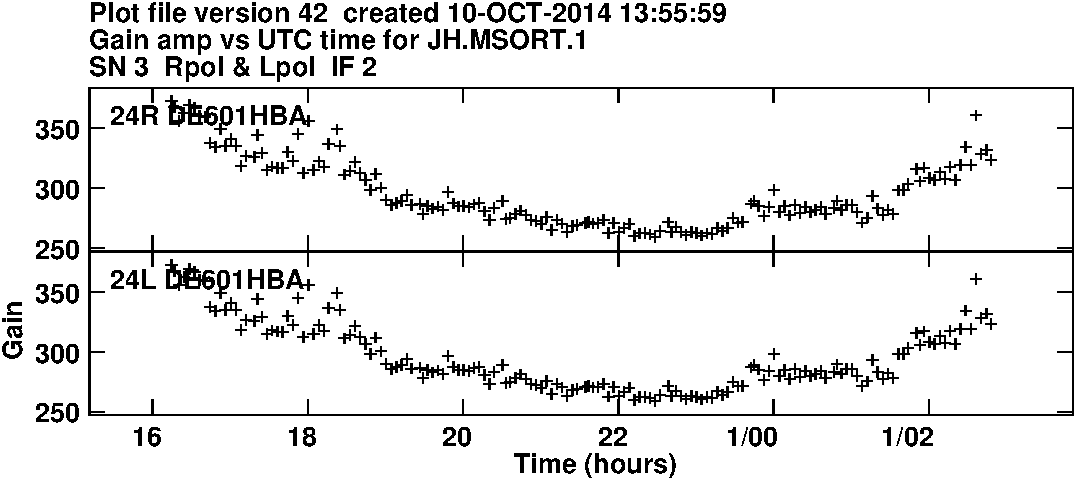
\includegraphics[width=0.8\textwidth]{figs/J0958Hampsols-crop.pdf}
    \label{fig:J0958Hamps}
}
\subfigure[Phase corrections for DE601HBA IF2]{
    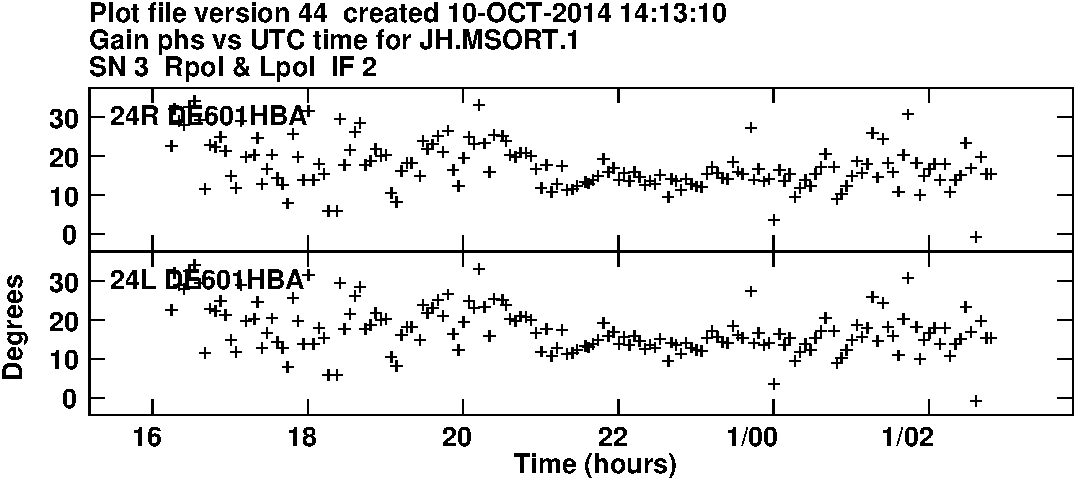
\includegraphics[width=0.8\textwidth]{figs/J0958Hphase-crop.pdf}
    \label{fig:J0958Hphases}
}
\caption{
The amplitude and phase corrections derived by CALIB for the international
LOFAR station DE601HBA during the first 10 hours of project LC0\_026.  We see
larger, and more noisy, corrections at the beginning and end of the experiment,
as expected from the smaller projected station area at these times relative to
transit. 
\label{fig:ampcal}
}
\end{figure*}
    
The final result of calibration for this baseline can be seen in Fig. \ref{fig:vplot}.
\begin{figure*}[htbp]
\centering
    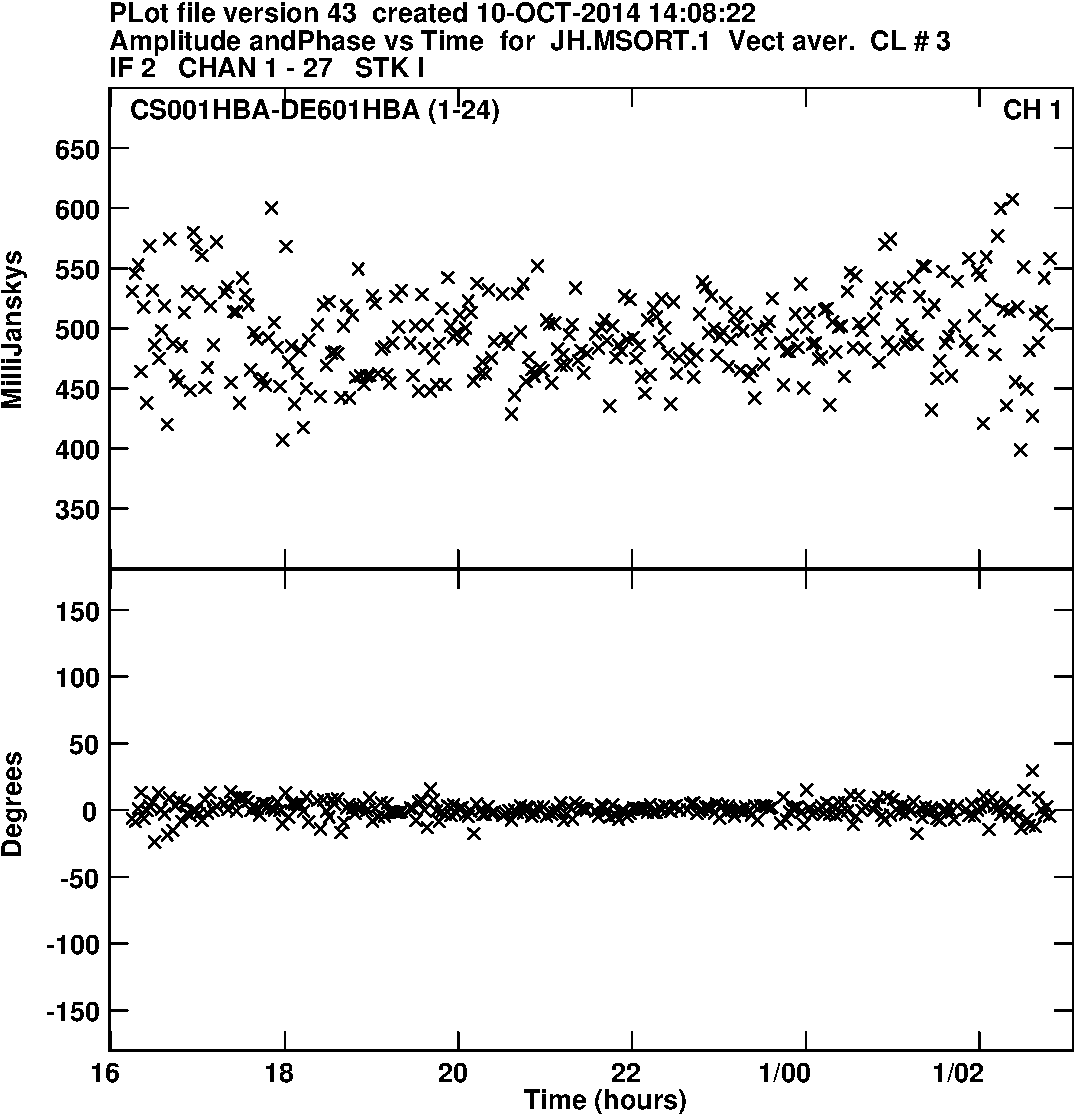
\includegraphics[width=0.8\textwidth]{figs/J0958Hvplot-crop.pdf}
\caption{
The final visibility amplitudes and phases on the DE601HBA-core baseline. We
assumed this source to be a 0.5Jy point source, which means that we should now
see two straight lines in this plot: one for the amplitude centered at
500\,mJy, and one for the phase centered at 0 degrees. This is also what we see
using VPLOT in AIPS to inspect the data. Apart from noise, there are marginal
changes differences to a point source. It is clear from \cite{varenius2014}
that this object has a weak extension to the south-west, and this should create
minor deviations in the visibilites compared to those of a point source.
\label{fig:vplot}
}
\end{figure*}

These solutions were now transferred to 3C196, which was imaged using NL-baselines only
to check the flux scale. More details by \cite{varenius2014}.

\subsection{ParselTongue - Scripting AIPS with python}
\label{sect:parseltongue}
TODO: Brief section with examples and ref on ParselTongue scripting. In practice,
I rarely use pure AIPS nowadays, almost all through ParselTongue / Eskil

\subsection{High-resolution imaging}
%- Brief comments on high-resolution imaging.
Although AIPS can determine delays and rates, it is not the best option for
imaging long baseline LOFAR data. Since we consider asmall field of view, we do
not need the beam models offered by AW-imager. However, at subarcsecond
resolution we will may need to take into account any effects of a non-coplanar
array, i.e. W-projection. The field of view $\theta_\mathrm{f}$ possible to
image without W-projection (i.e. using a single tangent plane) can be estimated
as $\theta_{\mathrm{f}} = \sqrt{\theta_{\mathrm{b}}}/3$ (see 2-29 in
\cite{NRAO}) where $\theta_\mathrm{b}$ is the FWHM of the synthesized beam,
both $\theta$ in radians. This expression assumes that we may tolerate phase errors
from no-coplanar effects of up to 0.1 radians in our image.
If your field to image is larger than this you need to
perform deconvolution using W-projection, for example in CASA.

\subsection{Combining the core into a single superstation}
\label{sect:phaseup}
%- How to form a sensitive tied station from the LOFAR core stations.
TODO: This section chould include parset files, background info about strong
calibrator and also plot of the station beam producet by the phased up core.
Eskil's calculations at 154MHz suggest 5\% amplitude loss at 30$''$ distance
from phase center, which is the most serious of all effects mentioned in this
document regarding field of view. Also, it is not clear to me if NDPPP
phase-rotates the data properly when adding the beams in a specific direction,
if using the shift-average approach in the coming pipeline.

\section{Scheduling long baseline LOFAR observations}
\label{sect:sched}
TODO: Maybe good to summarise how to select calibrators, subbands etc.?



\begin{thebibliography}{1}
\bibitem{NRAO} {Taylor}, G.~B. and {Carilli}, C.~L. and {Perley}, R.~A.{\em Synthesis Imaging in Radio Astronomy II}, ASPCS 180, 1999.
\bibitem{varenius2014} E. Varenius et al, {\em Subarcsecond international LOFAR radio images of the M82 nucleus at 118 MHz and 154 MHz}, submitted to A\&A.
\bibitem{vanhaarlem2013} {van Haarlem}, M.~P.  et. al. {\em LOFAR: The LOw-Frequency ARray}, A\&A 556A, 2V 2013
\bibitem{thompson} Thompson, A. R., Moran, J. M., \& Swenson, G. W. 2001, Interferometry and Synthesis in Radio Astronomy; 2nd ed. (Weinheim: Wiley-VCH)
\bibitem{skamemo113}R.J. Nijboer, M. Pandey-Pommier, A.G. de Bruyn, SKA memo 113: LOFAR imaging capabilities and system sensitivity, July, 2009.

\end{thebibliography}

\end{document}

